\documentclass[]{article}

\usepackage[german]{babel}
\usepackage{graphicx}
\usepackage{listings}
\usepackage{color}
\usepackage{subcaption}

\definecolor{gray}{rgb}{0.5,0.5,0.5}
\definecolor{orange}{RGB}{255,152,0}
\definecolor{green}{RGB}{76,175,80}

\lstset{frame=tb,
	aboveskip=5mm,
	belowskip=5mm,
	showstringspaces=false,
	columns=flexible,
	basicstyle={\small\ttfamily},
	numbers=left,
	numberstyle=\tiny\color{gray},
	breaklines=true,
	breakatwhitespace=false,
	tabsize=4
}

\lstset{
	language=C++,
	keywordstyle=\color{orange},
	stringstyle=\color{green},
	commentstyle=\color{gray}
}

%opening
\title{Private Information Retrieval}
\author{Ida Hönigmann}

\begin{document}

\maketitle

\begin{abstract}

\end{abstract}

\section{Idee}
In diesem Projekt wird ein System entwickelt bei dem Clients Nachrichten von verschiedenen Servern abfragen können. Die Besonderheit liegt in der Sicherheit, die dem Client gewährleistet wird: keiner der Server weiß welche Nachricht der Client lesen möchte.

Eine Möglichkeit diese Sicherheit umzusetzen ist es den Client alle Nachrichten abfragen zu lassen. Dieses Projekt wählt allerdings einen anderen Ansatz, der eine geringere Menge an Daten, die übertragen werden müssen ermöglicht. Der Nachteil ist, dass ein Client jeweils Anfragen an zwei Server stellen muss. Daher müssen zumindest zwei Server existieren, um Nachrichten empfangen zu können.

\section{Anwendungsfälle}
Dieses System ist für alle Systeme der Form von Servern, die Clients Nachrichten anbieten anwendbar.

Denkbar wäre zum Beispiel eine solche Lösung bei Daten zu Krankheiten. Wenn ein Benutzer nach einer Krankheit sucht, von der er weiß oder befürchtet diese zu haben, möchte er eventuell nicht, dass der Betreiber des Servers Kenntnis davon hat. Das gilt jedoch auch für Personen, die die Krankheit nicht haben und Informationen darüber erhalten wollen. Es könnte angenommen werden, dass sie die Krankheit besitzen, da sie ja danach gesucht haben.

Ein zweiter Anwendungsfall wäre ein Online-Nachrichtendienst. Oft wird nicht dediziert das Verhalten der Nutzer analysiert, sondern nur Logdaten gesammelt um Analysen über die Auslastung der Systeme zu erstellen oder falls ein Problem auftritt dieses nachverfolgen zu können. Jedoch kann es vorkommen, dass eine andere Organisation diese Logdaten anfordert um Informationen über einen bestimmten Benutzer oder eine Benutzergruppe erlangen zu können. Dazu muss die Organisation, die die Daten anfordert in irgendeiner Form über mehr Macht verfügen. Dies ist zum Beispiel bei Regierungen, auch anderer Länder, der Fall.

In diesen beiden und vielen anderen Fällen kann eine Implementierung eines \textit{private information retrieval} die Benutzer schützen.

\section{Funktionsweise}
Die in diesem Projekt implementierte Version von \textit{private information retrieval} nutzt die Eigenschaften der Exklusiv-Oder-Operation (xor).

\subsection{Exlusiv-Oder-Operation (xor)}
Die xor Operation erhält, gleich der ''und''- (Englisch ''and'') und der ''oder''- (Englisch ''or'') Operation zwei Signale als Eingang und liefert ein Signal als Ausgang. Dabei kann man das Verhalten von xor als ''entweder oder'' beschreiben. Die Wahrheitstafel in Tabelle~\ref{tab:wahrheitstafel_xor} definiert das Verhalten von xor genauer.

Die Eigenschaft, die dieses Projekt benötigt ist folgende: Jede Folge von Bytes $a$ mit einer anderen Folge von Bytes $b$ nach Anwendung der xor-Operation ergibt eine Folge von Bytes $c$ für die gilt, dass $c$ xor $a = b$ und $c$ xor $b = a$.

\begin{table}[]
	\centering
	\begin{tabular}{|l|l|l|}
		\hline
		\textbf{a} & \textbf{b} & \textbf{a xor b} \\ \hline
		0          & 0          & 0                \\ \hline
		0          & 1          & 1                \\ \hline
		1          & 0          & 1                \\ \hline
		1          & 1          & 0                \\ \hline
	\end{tabular}
	\caption{Wahrheitstafel der xor-Operation}
	\label{tab:wahrheitstafel_xor}
\end{table}

\subsection{Inhalt der gesendeten Nachrichten}
Ein Client baut zwei Verbindungen zu unterschiedlichen Servern auf. Statt nur die gewünschte Nachricht anzufordern, verlangt er das Produkt von xor-Operationen vieler Nachrichten.

Welche Nachrichten der Client anfordert, die Reihenfolge der Nachrichten, sowie die Anzahl sind irrelevant, solange beide Server die fast die gleichen Nachrichten verwenden. Der einzige Unterschied darf darin liegen, dass in einer der beiden Anforderungen die gewünschte Nachricht enthalten ist, und in der anderen Anforderung nicht.

Beide Server schicken dann das geforderte Produkt der Nachrichten zurück.

\subsection{Kalkulation der gewünschten Nachricht}
Der Client muss nun ebenfalls die xor-Operation auf die beiden erlangten Antworten der Server anwenden. Das Ergebnis ist die gewünschte Nachricht.

\section{Möglichkeiten einer Untergrabung}

\section{Implementation}
\subsection{Command Line Interface}
Das Command Line Interface wurde mit CLI11 umgesetzt.

Um Informationen über die Verwendung der beiden Programme \textit{client} und \textit{server} zu erhalten kann die Option $--help$ (oder als Kurzform $-h$) spezifiziert werden.

Sonstige Optionen, die bei \textit{client} spezifiziert werden können sind:

\begin{itemize}
	\item $--list$ / $-l$: gibt eine Liste aller Nachrichten Titel und deren Index aus
	\item $--index$ / $-i$: gibt die Nachricht des Index aus
	\item $--port1$ / $-p$: Port des ersten Server an dem die Nachrichten angefordert werden sollen
	\item $--server1$ / $-s$: IP Adresse des ersten Server an dem die Nachrichten angefordert werden sollen
	\item $--port2$ / $-q$: Port des zweiten Server an dem die Nachrichten angefordert werden sollen
	\item $--server2$ / $-t$: IP Adresse des zweiten Server an dem die Nachrichten angefordert werden sollen
	\item $--verbose$ / $-v$: gibt zusätzliche Debug Meldungen aus
\end{itemize}

\noindent
Die Optionen bei \textit{server} sind folgende:

\begin{itemize}
	\item $--port$ / $-p$: Port, an dem die Verbindung aufgebaut werden soll
	\item $--verbose$ / $-v$: gibt Debug Meldungen aus
	\item $--loop$ / $-l$: lässt den Server in einer Schleife laufen
	\item $--file$ / $-f$: Datei, in der die Nachrichten gespeichert sind
	\item $--size$ / $-s$: maximale Länge einer Nachricht
\end{itemize}

\subsection{Debug Ausgabe}
Wenn die \textit{verbose} Option beim Start des Servers oder des Clients angegeben wird, werden Debug Nachrichten ausgegeben. Der Server meldet so zum Beispiel wie viele Nachrichten er aus dem Datenfile eingelesen hat, den derzeitigen Verbindungsstatus und welche Nachrichten er gesendet hat. Beim Client wird zusätzlich zur Nachricht die jewilige Veränderung des Verbindungsstatus zu den zwei Servern ausgegeben.

Die Ausgabe der Debug Nachrichten wird mit spdlog umgesetzt.

\subsection{Fehler und Exitcodes}
Es gibt eine Reihe an Fehlerfällen, die bei der Verwendung dieses Programmes auftreten können. Pro Fehlerfall ist ein Exitcode, wie in Tabelle~\ref{tab:exit_codes} festgelegt.

\begin{table}[]
	\centering
	\begin{tabular}{|l|l|l|}
		\hline
		\textbf{Exitcode} & \textbf{Name} & \textbf{kann gesetzt werden von} \\ \hline
		0          & SUCCESS                & Client und Server     \\ \hline
		1          & SERVER\_UNREACHABLE    & Client                \\ \hline
		2          & DATA\_FILE\_NOT\_FOUND & Server                \\ \hline
		3          & ILLEGAL\_FILE\_FORMAT     & Server                \\ \hline
		4          & COULD\_NOT\_PARSE\_RESPONSE      & Client                \\ \hline
		5          & UNEXPECTED\_CLOSE      & Client und Server     \\ \hline
	\end{tabular}
	\caption{Auflistung aller Fehlercodes.}
	\label{tab:exit_codes}
\end{table}

\subsection{Aufbau und Speicher der Daten}
Da sich dieses Projekt auf die sichere Kommunikation fokussiert werden die Daten einfachheitshalber in einem Textfile gespeichert. Die Datei \textit{data.txt} wird als Datenspeicher verwendet. Der Aufbau der Daten ist abwechselnd der Titel der Nachricht und dann die eigentliche Nachricht. Da in dem Text der Daten prinzipiell alle Zeichen vorkommen können wird als Trennzeichen ein Zeilenumbruch (\textbackslash n) verwendet.

Das Datenfile wird ausgelesen nachdem der Server gestartet wurde.

\subsection{Byte-Operationen}
\label{sec:byte_operationen}
Um xor auf zwei Strings anwenden zu können wurde ein entsprechender Code in der Funktion \textit{xor\_string} implementiert.

\begin{lstlisting}
/* Perform xor on every char and return a new output char[]
* */
char* xor_string(const char a[], const char b[], unsigned int len=281) {
	char* output = new char[len];
	
	for (int i{}; i < len - 1; i++) {
		char tmp = a[i] ^ b[i];
		output[i] = tmp;
	}
	output[len - 1] = '\0';
	return output;
}
\end{lstlisting}

Da die zwei Array-von-Character-Parameter implizit auf Pointer des jeweils ersten Elements geändert werden, muss die Länge der Arrays als Parameter mitgegeben werden.

Die xor-Operation zweier Strings kann gelöst werden, indem jedes Zeichen (jeder Character) des Strings mit dem dazugehörigen Zeichen des anderen Strings xor verknüpft wird. Wenn das für alle Zeichen gemacht wird erhält man, durch zusammenfügen zu einem neuen String, das Ergebnis.

Zwei Character in C++ xor zu verknüpfen ist relativ einfach, da ein Character immer gleich lange ist (meist 8 Bit = 1 Byte). In Zeile 7 wird diese xor Verknüpfung vorgenommen. Nachdem alle Zeichen xor-verknüpft sind (also Zeile 7 \textit{len - 1} Mal durchgeführt wurde) wird zuletzt noch ein \textbackslash 0 hinzugefügt. Dieses markiert für gewöhnlich das Ende eines Strings.

Die Funktion liefert einen Pointer auf ein Characterarray zurück, da alle anderen Rückgabetypen, die normalerweise in solch einer Situation verwendet werden könnten, Probleme verursacht haben. Das Problem, das bei einem xor von zwei gleichen Zeichen auftritt ist, dass das Ergebnis \textbackslash 0 ergibt. Das wird in Abbildung~\ref{fig:xor_gleiches_zeichen} gezeigt. Bei allen Stringoperationen wird allerdings das \textbackslash 0 als Ende angesehen, daher musste direkt in einigen Bereichen direkt auf den Speicher zugegriffen werden.

\begin{table}[]
	\centering
	\begin{tabular}{l|l}
		Bitmuster  & Bedeutung (ASCII)\\ \hline
		01100001   & a                \\
		01100001   & a                \\ \hline
		00000000   & \textbackslash 0 \\
	\end{tabular}
	\caption{Zwei gleiche Zeichen (a) miteinander xor verknüpft ergibt das Bitmuster 00000000, welches \textbackslash 0 bedeutet. Dieses Symbol steht normalerweise nur am Ende eines Strings.}
	\label{fig:xor_gleiches_zeichen}
\end{table}

Eine Bedingung um die \textit{xor\_string} Funktion anwenden zu können ist, dass beide Strings gleich lange sein müssen. Selbst wenn die beiden Strings als Character-Array mit der gleichen Größe angelegt werden gibt es Probleme. Um effizient zu sein, wird beim Initialisieren eines Character-Arrays nur der Teil beschrieben, der auch verwendet werden muss. So kann zum Beispiel folgender Code

\noindent
\lstinline|char* char_ptr = new char[10]; strcpy(char_ptr, "Hello!");| das Bitmuster in Abbildung~\ref{fig:bitcode_char_array} ergeben.

\begin{table}[]
	\centering
	\begin{tabular}{l|l}
		Bitmuster  & Bedeutung (ASCII)\\ \hline
		01001000   & H                \\
		01100101   & e                \\
		01101100   & l                \\
		01101100   & l                \\
		01101111   & o                \\
		00100001   & !                \\
		00000000   & \textbackslash 0 \\
		00001001   & TAB              \\
		00000000   & \textbackslash 0 \\		
		01000001   & A                \\		
	\end{tabular}
	\caption{Das Bitmuster, das nach Ausführung des Codes \lstinline|char* char_ptr = new char[10]; strcpy(char_ptr, "Hello!");| beispielsweise im Speicher stehen kann.}
	\label{fig:bitcode_char_array}
\end{table}

Wenn nun zwei Strings mit einer unterschiedlichen Anzahl an Zeichen an die \textit{xor\_string} Funktion übergeben werden, entsteht nach dem letzten Zeichen des kürzeren Texts eine zufällige Zeichenfolge und die längere Nachricht kann vom Client nicht mehr gelesen werden.

Um das zu vermeiden füllt die Funktion \textit{cleanup\_char\_arr} die Zeichen nach dem \textbackslash 0 mit Leerzeichen auf. Um den resultierenden String weiter wie jeden andren String behandeln zu können wird zuletzt das \textbackslash 0 auf der letzten Position gesetzt.

\begin{lstlisting}
/* Sets all chars after (and including) the \0 to spaces
* to enable all xor operations to be performed smoothly;
* (and sets the \0 back into the last char)
* */
void cleanup_char_arr(char a[], unsigned int len=281) {
	std::fill(a + strlen(a), a + len - 1, ' ');
	a[len - 1] = '\0';
}
\end{lstlisting}

\subsection{Zufällige Nachrichten anfordern}
Um die Sicherheit des Client zu garantieren müssen zufällige Nachrichten angefordert werden. Weiters muss die Anzahl der Nachrichten zufällig sein, da sonst ein Server feststellen könnte, das eine der von ihm verlangten Nachrichten, die ''richtige'' ist. Zusätzlich müssen die Nachrichten in einer zufälligen Reihenfolge angefordert werden. Wenn zum Beispiel die ''richtige'' Nachricht immer die erste wäre, hätte der Server ein leichtes Spiel.

Um all diese Anforderungen umzusetzten wird in diesem Projekt die \textit{random}-Bibliothek verwendet.

\begin{lstlisting}
/* setup number distributions */

random_device seeder;
mt19937 rndm_engine{seeder()};

uniform_int_distribution<int> dist_idx(0, stoi(cnt_messages) - 1);
uniform_int_distribution<int> dist_cnt(5, 10);

int cnt{dist_cnt(rndm_engine)};     /* number of messages to request */
for (int i{}; i < cnt; i++) {
	int num{message_idx};
	while (find(req_idx.begin(), req_idx.end(), num) != req_idx.end()) {
		num = dist_idx(rndm_engine);
	}
	req_idx.push_back(num);     /* message idx to request */
}
\end{lstlisting}

Dieser Code erfüllt die ersten beiden Anforderungen (zufällige Anzahl an zufälligen Nachrichten). Zuerst wird, in Zeile 9, die Anzahl der Nachrichten festgelegt. Diese ann einen Wert zwischen 5 und 10 annehmen. In der darauffolgenden Schleife werden so lange zufällige Zahlen generiert, bis diese noch nicht in \textit{req\_idx}, einem Vector der die Nachrichten Indizes speichert, enthalten sind. Dabei kann jede Zahl zwischen 0 und der Anzahl der Nachrichten weniger Eins hinzugefügt werden.

Das zufällige Umordnen des Vectors wird mit folgender Zeile Code erreicht:

\begin{lstlisting}
/* randomize the oder of the requested messages */

shuffle(begin(idx_), end(idx_), rndm_engine);
\end{lstlisting}

Dabei steht \textit{idx\_} für eine Kopie von \textit{req\_idx}. Damit wird der originale Vektor nicht verändert.

\subsection{Kommunikation}
Die Kommunikation zwischen allen beteiligten Einheiten wird über asio geregelt. Asio ermöglicht eine einfache Kommunikation über Streams.

Die zwei typischen Kommunikationsabläufe werden in Abbildung~\ref{fig:communication_diagram} gezeigt.

\begin{figure*}[t!]
	\centering
	\begin{subfigure}[t]{0.5\textwidth}
		\centering
		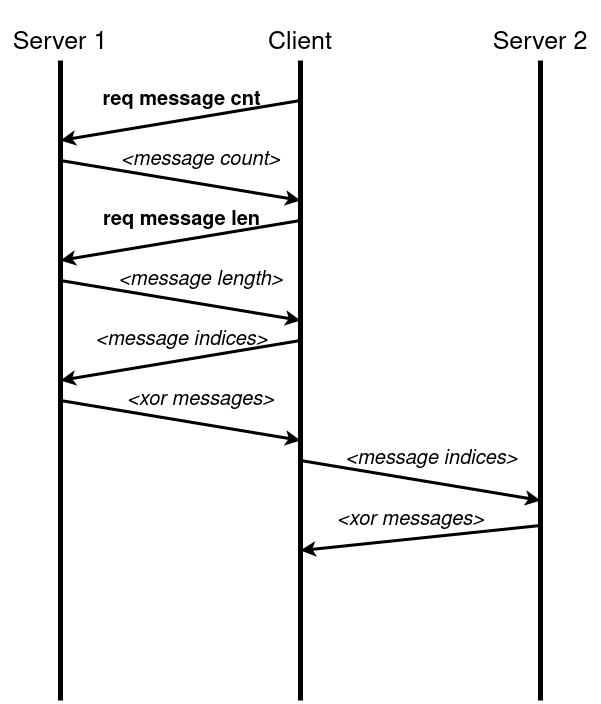
\includegraphics[height=7cm]{img/communication_index.png}
		\caption{Eine Nachricht wird abgefragt. Dazu muss der Client zuerst die Anzahl der Nachrichten, sowie deren Länge wissen. Dann fragt er beide Server nach bestimmten Nachrichten, die dann xor-verknüpft zurückgesendet werden.}
	\end{subfigure}%
	~ 
	\begin{subfigure}[t]{0.5\textwidth}
		\centering
		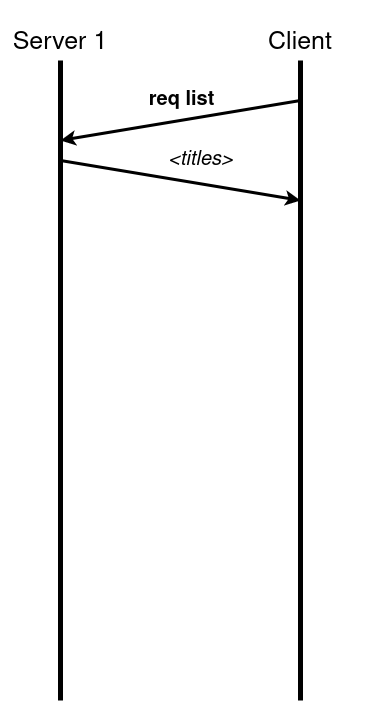
\includegraphics[height=7cm]{img/communication_list.png}
		\caption{Client fragt die Nachrichtentitel ab.}
	\end{subfigure}
	\caption{Die zwei gewöhnlichen Kommunikationsabläufe.}
	\label{fig:communication_diagram}
\end{figure*}

Der einzige Codeteil, bei dem der asio-stream nicht wie gewohnt, um Strings einzulesen und zu versenden, verwendet wird ist bei der Übermittlung des eigentlichen Dateninhalts. Da bei den Daten, wie in Abschnitt~\ref{sec:byte_operationen} beschrieben, das Zeichen \textbackslash 0 vorkommen kann, können hier nicht gewöhnliche Stringfunktionen verwendet werden. Stattdessen wird auf Senderseite folgender Code verwendet:

\begin{lstlisting}
/* send data */

spdlog::debug("sending {}", data);
strm.write(output, message_len + 1);
\end{lstlisting}

Auf der Empfängerseite sieht das Gegenstück folgendermaßen aus:

\begin{lstlisting}
/* receive data */

string data;
char* buffer = new char[message_len + 1];

/* write messages into char buffer */

while (strm.read(buffer, sizeof(buffer))) {
	data.append(buffer, sizeof(buffer));
}

/* move buffer into string */

data.append(buffer, strm.gcount());

delete[] buffer;
spdlog::debug("received data");
\end{lstlisting}

Diese beiden Codeabschnitte ermöglichen es, statt wie normalerweise Daten, deren Ende durch ein \textbackslash n oder \textbackslash 0 gekennzeichnet sind, eine fixierte Länge an Bytes zu schreiben und auszulesen. Die Anzahl an geschriebenen und ausgelesenen Bytes ist durch die Nachrichtenlänge (\textit{message\_len}) definiert. Diese wird um Eins erhöht, da die Nachricht durch ein \textbackslash 0 beendet ist.

Um die erhaltenen Daten zu speichern, werden diese in einen Vector angehangen. Da die Daten später als Characterarray vorliegen müssen, werden sie hier konvertiert. Das stellt auch sicher, dass keine Probleme mit \textbackslash 0 auftreten.

\begin{lstlisting}
/* copy messages viy memcpy to avoid \0 stopping the copy process */

char* answer = new char[message_len + 1];
memcpy(answer, data.c_str(), message_len + 1);
responses.push_back(answer);
\end{lstlisting}

Um die Daten ohne Verlust von allem, das hinter dem ersten \textbackslash 0 steht in ein Characterarray kopieren zu können, muss die Funktion \textit{memcpy} verwendet werden. Diese kopiert die Bytewerte von Beginn des \textit{data.c\_str()} Pointers auf den Speicherbereich des \textit{answer} Pointers für \textit{message\_len} + 1 Bytes.

\end{document}
